\section{Rigid Body Simulation}
\tododone[inline]{Benni}{responsible for section \textbf{RB}: Friedrich}

The goal of this project was to develop a game which is based on a real time physics simulation for fluid flow, rigid bodies as well as their interaction. The main task of the rigid body group was hence the collision detection and collision handling between the different objects, while the interface to the fluid group gives us the necessary interaction from the fluid on the bodies and vice versa. While the interaction between simple shapes like circles and rectangles is manageable, it becomes more complex for polygons. Therefore, whereas the fluid group implemented their own LBM solver, we decided to adapt the real-time physics library Bullet \cite{Bullet} for the rigid body handling. By doing this, we did not have to invent the wheel anew. Furthermore, Bullet gives a lot of possibilities for extensions to the program offering a variety of different complex shapes for example. Hence, the first approach was to implement Bullet using simple shapes, such as circles and rectangles and then move on to more complex polygons.
%\begin{itemize}
%\item simulation driven game one half LBM, one half RB
%\item RB simulation is very simple for circles, becomes more complicated for rectangles and gets a real problem for polygons and other complex stuff. Our strategy: Wrap a fully developed RB engine and use its functionality
%\item the main problem is not the implementation of the functionality, but the interfaces!
%\end{itemize}

\subsection{Bullet}
As a consequence, our first task in this project was to get Bullet running on multiple layers-- i.e. understanding the library as well as using it in our project. This task, as simple as it might seem at first sight, already included some pitfalls, which we hope to diminish for the next group with the help of this report. 
\subsubsection{Building}
To build bullet, you need cmake \cite{CMake}. After having downloaded the Bullet library from their webpage, one can follow the instructions below to build the library:
\begin{enumerate}
\item Extract the \verb+fa/sources-for-rigidbody/bullet3-2.83.6.tar.gz +
\item run \verb+cmake . + in the top directory.
\item run \verb+make -j4+ (\verb+-j4+ chooses 4 threads for compilation) in the top directory.
\item run \verb+sudo make install + in the \verb+src+ directory.
\end{enumerate}
Afterwards, link to the library in your compilation (usually \verb+/usr/local/include/bullet+ and \verb+-L/usr/local/lib+)
\subsubsection{Functionality we used}
We had three basic classes from Bullet which we used. The first was \verb+btDiscreteDynamicsWorld+, see \autoref{fig: btDDWgraph}. As the class name already states, \verb+btDiscreteDynamicsWorld+ can be seen as the world where the rigid body simulation takes place. It contains all the rigid bodies and all important world parameter, like gravity and size of a timestep for example. By calling \verb+stepSimulation()+ on the world, Bullet performs one simulation step on all the rigid bodies in the world.
\begin{figure}
\centering
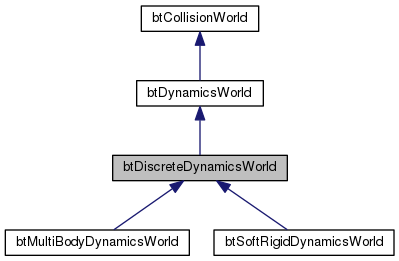
\includegraphics[scale=0.5]{img/RigidBodies/btDiscreteDynamicsWorldGraph.png}
\caption{Inheritance diagram of \texttt{btDiscreteDynamicsWorld}}
\label{fig: btDDWgraph}
\end{figure}


With that, we directly come to rigid body class from Bullet which we used: \verb+btRigidBody+, see \autoref{fig: btRBgraph}. It is the main class of Bullet for rigid body objects. The library offers three kinds of rigid bodies types:
\begin{enumerate}
\item Dynamic rigid bodies, with positive mass. Motion is controlled by rigid body dynamics.
\item Fixed objects with zero mass. They are not moving (basically collision objects)
\item Kinematic objects, which are objects without mass, but the user can move them
\end{enumerate}
We used objects of type 1. and 2., which we controlled by assigning them the corresponding mass. Hence, we could build dynamic (floating obstacles) and static objects (walls, boundaries) in our simulation. Furthermore, the \texttt{btRigidBody} class offers methods to access the properties of the objects such as 
\begin{itemize}
\item \texttt{getTotalForce():} Returning the force applied on the object
\item \texttt{getLinearVelocity():} Returning the linear velocity
\item \texttt{getCenterOfMass():} Returning the current center of mass
\end{itemize}
to name a few. 
\begin{figure}
\centering
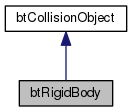
\includegraphics[scale=0.5]{img/RigidBodies/btRigidBodyGraph.png}
\caption{Inheritance diagram of \texttt{btRigidBody}}
\label{fig: btRBgraph}
\end{figure}


Finally, Bullet also offers the possibility to assign a shape to a \texttt{btRigidBody} object. Here, a shape object can be rather seen as a pattern than an actual object, since multiple rigid bodies can share the same shape object. The class in Bullet is called \texttt{btCollisionShape}. See \autoref{fig: btCSgraph} in the appendix, for an inheritance diagram which shows the amount of different shapes this family of classes provides. From convex shapes over concave shapes to compound shapes which one can design by himself. The two shapes that we use are \texttt{btCylinderShape} and \texttt{btBoxShape}, see \autoref{fig: btCylSgraph} and \autoref{fig: btBoxSgraph}. By assigning a height of 1 to the cylinder we received a circle shape; the box shape was used for rectangles and squares. The idea was to later move on to more complex polygons, of course.
\begin{figure}[ht]
\centering
\begin{minipage}{.45\linewidth}
\centering
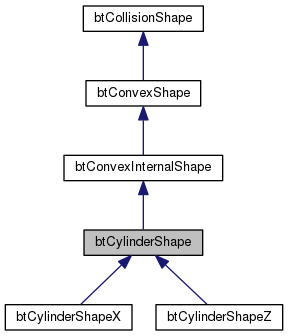
\includegraphics[scale=0.5]{img/RigidBodies/btCylinderShapeGraph.png}
\caption{Inheritance diagram of \texttt{btCylinderShape}}
\label{fig: btCylSgraph}
\end{minipage}
\hspace{.05\linewidth}
\begin{minipage}{.45\linewidth}
\centering
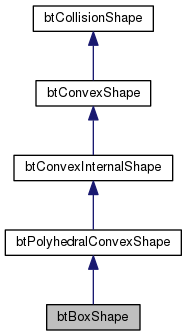
\includegraphics[scale=0.5]{img/RigidBodies/btBoxShapeGraph.png}
\caption{Inheritance diagram of \texttt{btBoxShapeGraph}}
\label{fig: btBoxSgraph}
\end{minipage}
\end{figure}

\subsubsection{Implementation}
In this section we want to take a look at our actual implementation. For that, the general structure is depicted with the help of an UML diagram, see \autoref{fig: RBUMLgraph}. Although the diagram shows a few of the most important methods, it focus lays more on the connection between the classes and the general structure. In the following, we want to give a simple introduction to the individual classes. All of them are also documented with the help of Doxygen \cite{Doxygen}. Hence, to get a more detailed informations about the properties, members and methods of each class, create the Doxygen documentation by calling \texttt{doxygen Doxyfile} in the top most folder of the source code. The main page of the documentation can then be found in \texttt{/html/index.html}.
\begin{figure}[ht]
\centering
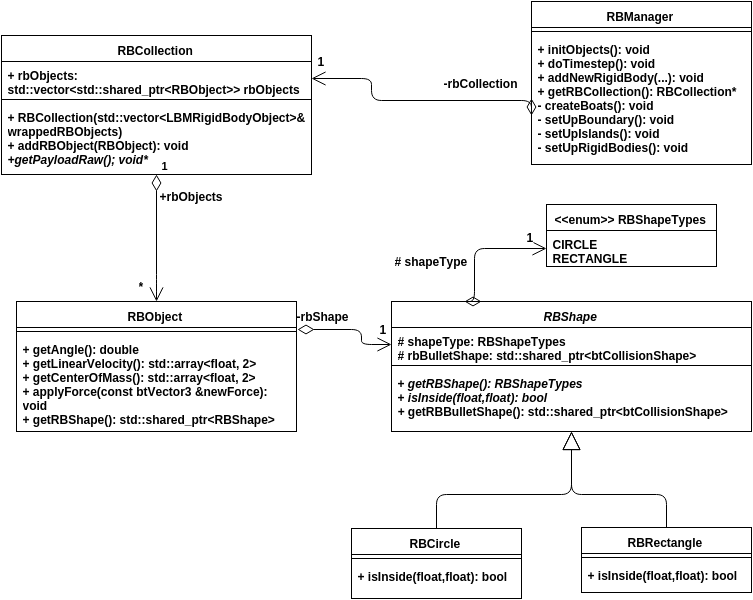
\includegraphics[scale=0.5]{img/RigidBodies/RigidBodyUML.png}
\caption{UML diagram of rigid body classes}
\label{fig: RBUMLgraph}
\end{figure}

\subsubsection*{RBObject and RBShape}
To wrap Bullet, we developed our own classes which we named \texttt{RBObject} and \texttt{RBShape}, which wrap \texttt{btRigidBody} and \texttt{btCollisionShape} respectively. The two specific shapes, we implemented by now are \texttt{RBCircle} and \texttt{RBRectangle}, see \autoref{fig: RBShape} for the specific inheritance diagram. \texttt{RBObject} on the other hand includes all the methods from Bullet which we need to transfer information for the LBM simulation and the visualization, like \texttt{getLinearVelocity()} and \texttt{getCenterOfMass()} as mentioned above. 
\begin{figure}[ht]
\centering
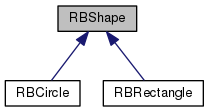
\includegraphics[scale=0.5]{img/RigidBodies/RBShapeGraph.png}
\caption{Inheritance diagram of \texttt{RBShape}}
\label{fig: RBShape}
\end{figure}

\subsubsection*{RBCollection}
We furthermore wrote a class \texttt{RBCollection} which is a container class for all generated \texttt{RBObjects}. \texttt{RBCollection} is also responsible for the communication to LBM and visualization, since it is a derived class from \texttt{CPipelinePacket}. With methods like 
\begin{itemize}
\item \texttt{getLBMOBjectWrapperBegin()}
\item \texttt{getPayloadRaw()}
\end{itemize} 
it gives access to different informations transferred between the stages. 

\subsubsection*{RBManager}
\label{sec: rbManager}
The class \texttt{RBManager} has a \texttt{btDiscreteDynamicWorld} as member, control over the \texttt{RBCollection} and is hence responsible for the simulation. By calling the class method \texttt{doTimeStep()} one implicitly calls the method \texttt{stepSimulation()} of \texttt{btDiscreteDynamicWorld}. Furthermore, \texttt{RBManager} is responsible for setting up the correct world with the help of the methods by using its interface to image recognition (see \autoref{sec: interfaceImageRecognition}:
\begin{itemize}
\item \texttt{addNewRigidBody():} Adds a new rigid body to \texttt{RBCollection} and \texttt{btDiscreteDynamicWorld}.
\item \texttt{setUpIslands():} Sets up the islands sent from image recognition.
\item \texttt{setUpBoundary():} Sets up the boundary sent from image recognition.
\item \texttt{setUpRigidBodies():} Sets up the floating objects in the domain sent from image recognition.
\item \texttt{createBoats():} Sets up the boats based on the position given by image recognition.
\end{itemize}

\subsubsection{Discussion}
\tododone[inline]{Benni}{responsible for \textbf{Discussion} on RB and Bullet: Erik, Friedrich, Benni}
\begin{itemize}
\item was a bit of an overkill: in the end we only used circles anyhow.
\item better way: 
\begin{itemize}
\item first simple mock up with basic, easy functionality implemented on our own: explicit euler, circles, no performance optimization...
\item then wrap physics engine as soon as interfaces are defined and running, whole change under the hood
\end{itemize}
\end{itemize}

\subsection{Interfaces}
\tododone[inline]{Benni}{responsible for subsection \textbf{Interfaces} of RB: Friedrich}
As it turned out during the project, the actual more complex task was to get the interfaces running between the different groups. Rigid bodies needed interaction with all of them:
\begin{itemize}
\item \textbf{Input devices:} Boat is a rigid body and forces are applied from input devices
\item \textbf{Image recognition:} Sends the terrain information which is then implemented as rigid bodies
\item \textbf{Visualization:} Correct visualization of objects depending on their properties
\item \textbf{LBM:} Fluid-structure interaction between flow and objects
\end{itemize}
Hence, the correct implementation of the interfaces was an important task, since if they are not working the whole project gets stuck. In the following sections, we want to explain the implementations of the different interfaces to the other groups in more detail.
%\begin{itemize}
%\item RB have many interfaces! Most complex to LBM, but also many more interfaces with different demands.
%\item discrete version(LBM, ImgRecognition) vs. continuous version(Visu, RB Internal) of RBs
%\end{itemize}
\subsubsection{to Input Devices}
\tododone[inline]{Benni}{responsible for interface from RB \textbf{to Input Devices}: Erik?}
\begin{itemize}
\item how to model rowing
\item apply forces to bodies depending on input
\item in the end more time for finetuning would have been good!
\end{itemize}
\subsubsection{to Image Recognition}
\label{sec: interfaceImageRecognition}
\tododone[inline]{Benni}{responsible for interface from RB \textbf{to Image Recognition}: Friedrich}
The interface to image recognition works with the help of the \texttt{ProcessingManager} class (as also already described in \autoref{sec: imageProcessing}) which we included as member in \texttt{RBManager}. This class contains all the information needed for us to set up the correct boat starting positions, boundaries, rigid and static bodies. The methods of \texttt{ProcessingManager} which we used were:
\begin{itemize}
\item \texttt{boatCenters(): std::vector<cv::Vec2f>} returning a 2D vector with the position of the boats.
\item \texttt{outerBorder(): Polygon} returning a \texttt{Polygon} which holds the structure of the outer border
\item \texttt{rigidBodies(): std::vector<Polygon>} returning all rigid bodies, stored as \texttt{Polygons}
\item \texttt{staticBodies(): std::vector<Polygon>} returning all static bodies, stored as \texttt{Polygons}
\end{itemize} 
The corresponding methods which calls them in \texttt{RBManager} were already described in \autoref{sec: rbManager}.


For each \texttt{Polygon} given from the \texttt{ProcessingManager}, we can now calculate a center of mass. For rigid bodies (static or dynamic) we calculated the mean position of the polygon points as center of mass $\overrightarrow{x}$ and also the mean deviation $\hat{r}$ to approximate a radius $r$. By connecting the polygon points one after another with the help of rectangular shaped rigid bodies, we set up the boundary. The mass and shape is assigned depending on the type of the body and its volume (mass=0: static body, mass$>$0: dynamic body). We end up with four different kinds of rigid bodies which we approximated.
\begin{itemize}
\item \textbf{Boats:} RBCircle with position $\overrightarrow{x}$, radius $r=20$, mass$=0.6e4$ and moment of inertia$=1.2e7$.
\item \textbf{Islands:} RBCircle with position $\overrightarrow{x}$, radius $r=\hat{r}$, mass$=0$ and moment of inertia$=0$.
\item \textbf{Floating Objects:} RBCircle with position $\overrightarrow{x}$, radius $r=\hat{r}$, mass$=r^2$, and moment of inertia $=0$.
\item \textbf{Boundary:} RBRectangle connecting points of polygon, mass$=0$ and moment of inertia $=0$.
\end{itemize}
In the end, these new objects are added to the \texttt{btDiscreteDynamicWorld} and to \texttt{RBCollection}.


As one can easily imagine there is a lot of freedom in the exact parameter choice; the values taken here were derived from playing the game and getting a user feedback.
%\begin{itemize}
%\item how to model boundaries
%\item how to create different rigid bodies
%\end{itemize}
\subsubsection{to Visualization}
\tododone[inline]{Benni}{responsible for interface from RB \textbf{to Visualization}: Benni?}
\begin{itemize}
\item represent shapes in an abstract way
\end{itemize}
\subsubsection{to LBM}
\tododone[inline]{Benni}{responsible for interface from RB \textbf{to LBM}: Erik?}
\begin{itemize}
\item how to send important quantities (discretization of continuous RB into cells, velocity of RB...)
\item how to receive important quantities (forces and torques from the fluid on the body)
\end{itemize}